\documentclass[class=article,border=0pt,varwidth]{standalone}
\usepackage{fancybox,pstricks,pst-node,tikz}

\begin{document}
  \pagestyle{empty}
  \thispagestyle{empty}
  \psset{linewidth=1.5pt,framearc=0.3}

\begin{tabular}{c c c c c}
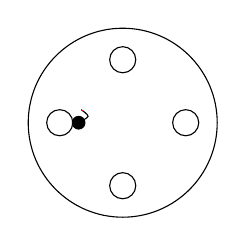
\begin{tikzpicture}[scale = 0.8]

\draw (0, 0) circle (1.5);

\node[draw, circle, fill=white] at (1, 0) {};
\node[draw, circle, fill=white] at (0, 1) {};
\node[draw, circle, fill=white] at (-1, 0) {};
\node[draw, circle, fill=white] at (0, -1) {};

\def\x{-0.7}
\def\y{0}
\draw[fill=black] (\x, \y) circle (0.1);
\draw plot [smooth] coordinates {(\x, \y) (\x + 0.15, \y + 0.1) (\x + 0.05, \y + 0.2) };
\draw[red, dotted] (\x + 0.05, \y + 0.2) -- (\x + 0.05 + 0.1, \y + 0.2);
\draw[red, dotted] (\x + 0.05, \y + 0.2) -- (\x + 0.05, \y + 0.2 + 0.1);
\draw[red, dotted] (\x + 0.05, \y + 0.2) -- (\x + 0.05, \y + 0.2 - 0.1);
\draw[red, dotted] (\x + 0.05, \y + 0.2) -- (\x + 0.05 - 0.1, \y + 0.2);

\end{tikzpicture}

&

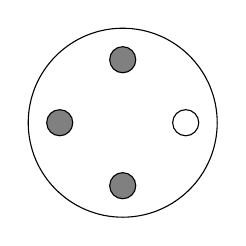
\begin{tikzpicture}[scale = 0.8]

\draw (0, 0) circle (1.5);

\node[draw, circle, fill=white] at (1, 0) {};
\node[draw, circle, fill=gray] at (0, 1) {};
\node[draw, circle, fill=gray] at (-1, 0) {};
\node[draw, circle, fill=gray] at (0, -1) {};
\end{tikzpicture}

&

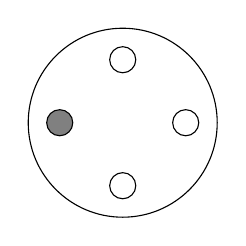
\begin{tikzpicture}[scale = 0.8]

\draw (0, 0) circle (1.5);

\node[draw, circle, fill=white] at (1, 0) {};
\node[draw, circle, fill=white] at (0, 1) {};
\node[draw, circle, fill=gray] at (-1, 0) {};
\node[draw, circle, fill=white] at (0, -1) {};
\end{tikzpicture}

&

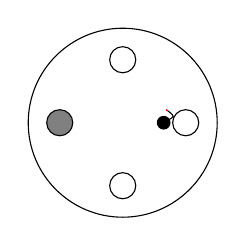
\begin{tikzpicture}[scale = 0.8]

\draw (0, 0) circle (1.5);

\node[draw, circle, fill=white] at (1, 0) {};
\node[draw, circle, fill=white] at (0, 1) {};
\node[draw, circle, fill=gray] at (-1, 0) {};
\node[draw, circle, fill=white] at (0, -1) {};

\def\x{0.65}
\def\y{0}
\draw[fill=black] (\x, \y) circle (0.1);
\draw plot [smooth] coordinates {(\x, \y) (\x + 0.15, \y + 0.1) (\x + 0.05, \y + 0.2) };
\draw[red, dotted] (\x + 0.05, \y + 0.2) -- (\x + 0.05 + 0.1, \y + 0.2);
\draw[red, dotted] (\x + 0.05, \y + 0.2) -- (\x + 0.05, \y + 0.2 + 0.1);
\draw[red, dotted] (\x + 0.05, \y + 0.2) -- (\x + 0.05, \y + 0.2 - 0.1);
\draw[red, dotted] (\x + 0.05, \y + 0.2) -- (\x + 0.05 - 0.1, \y + 0.2);


\end{tikzpicture}

&

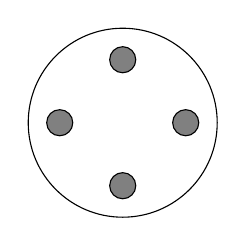
\begin{tikzpicture}[scale = 0.8]

\draw (0, 0) circle (1.5);

\node[draw, circle, fill=gray] at (1, 0) {};
\node[draw, circle, fill=gray] at (0, 1) {};
\node[draw, circle, fill=gray] at (-1, 0) {};
\node[draw, circle, fill=gray] at (0, -1) {};
\end{tikzpicture}

\\

first bomb

&

after the blast

&


after the boss moves

&

second bomb

&

after the blast

\end{tabular}

%% \begin{tikzpicture}[scale = 0.8]
%% \node[circle, fill=white] at (-11, 0.5) {};
%% \node[draw, circle, fill=gray] at (0, 0) {};
%% \node at (2.2, 0) {\small position where the};
%% \node at (1.9, -0.5) {\small boss cannot be};

%% \end{tikzpicture}

\end{document}
